% =====================================================================
%  Workshop 1 - Project Definition Report (IEEE conference layout)
%  Team 4 - Tropical Cyclone Monitoring
%  Data Analysis Programming 2026-II, Universidad Distrital FJC
%  Build: pdflatex workshop1_report.tex (run twice)
% =====================================================================
\documentclass[10pt,twocolumn,letterpaper]{article}

% ---------- page geometry (IEEE conference, US letter) --------------
\usepackage[letterpaper,top=0.75in,bottom=1in,left=0.625in,right=0.625in,columnsep=0.25in]{geometry}
\usepackage[T1]{fontenc}
\usepackage[utf8]{inputenc}
\usepackage{mathptmx}            % Times text and math
\usepackage[scaled=0.86]{helvet}
\usepackage{courier}
\usepackage{microtype}
\usepackage{amsmath}
\usepackage{graphicx}
\usepackage{array,booktabs,tabularx,multirow,makecell}
\usepackage{stfloats}            % bottom-placed double-column floats
\usepackage{balance}
\usepackage[hyphens]{url}
\makeatletter\g@addto@macro\UrlBreaks{\do\_\do\&\do\=\do\?\do\.}\makeatother
\usepackage[colorlinks=false,pdfborder={0 0 0},pdftitle={TC-Analog Monitor: Hazard Definition, Source Validation and Data Contract},pdfauthor={O. Pena, R. Lopez, B. Ramirez}]{hyperref}
\usepackage{listings}
\usepackage{xcolor}
\usepackage{titlesec}
\usepackage[font=footnotesize,labelsep=period]{caption}
\usepackage{enumitem}

% ---------- editable values ----------------------------------------
\newcommand{\repourl}{\url{https://github.com/<team>/tc-monitor}} % <-- replace with the real link

% ---------- IEEE-like headings --------------------------------------
\renewcommand{\thesection}{\Roman{section}}
\renewcommand{\thesubsection}{\Alph{subsection}}
\renewcommand{\thesubsubsection}{\arabic{subsubsection})}
\titleformat{\section}{\centering\normalsize\scshape}{\thesection.}{0.5em}{}
\titlespacing*{\section}{0pt}{10pt plus 2pt minus 2pt}{5pt plus 1pt}
\titleformat{\subsection}{\normalsize\itshape}{\thesubsection.}{0.5em}{}
\titlespacing*{\subsection}{0pt}{7pt plus 2pt minus 1pt}{3pt plus 1pt}
\titleformat{\subsubsection}[runin]{\normalsize\itshape}{\thesubsubsection}{0.4em}{}[:]
\titlespacing*{\subsubsection}{\parindent}{3pt}{0.5em}

% ---------- captions: "Fig. 1." below, "TABLE I" above ---------------
\renewcommand{\figurename}{Fig.}
\renewcommand{\thetable}{\Roman{table}}
\DeclareCaptionFormat{ieeetable}{\centering\textsc{#1}\\\textsc{#3}\par}
\DeclareCaptionLabelSeparator{ieeenone}{}
\captionsetup[table]{format=ieeetable,labelsep=ieeenone,skip=3pt,font=footnotesize,name=TABLE}
\captionsetup[figure]{skip=4pt,justification=justified,singlelinecheck=true}

% ---------- misc ----------------------------------------------------
\setlength{\parindent}{1em}
\setlist{nosep,leftmargin=1.4em}
\newcommand{\code}[1]{\texttt{\footnotesize #1}}
\renewcommand{\arraystretch}{1.12}
\setlength{\tabcolsep}{3.5pt}
\newcolumntype{L}[1]{>{\raggedright\arraybackslash}p{#1}}
\newcolumntype{Y}{>{\raggedright\arraybackslash}X}
\lstset{basicstyle=\ttfamily\scriptsize,breaklines=true,breakatwhitespace=false,
        columns=fullflexible,keepspaces=true,frame=tb,framerule=0.4pt,
        xleftmargin=2pt,xrightmargin=2pt,aboveskip=4pt,belowskip=4pt,
        literate={°}{{$^\circ$}}1}
\pagestyle{empty}
\renewcommand{\lstlistingname}{Listing}
\captionsetup[lstlisting]{font=footnotesize,labelsep=period,justification=centering,singlelinecheck=false,skip=2pt}
\urlstyle{same}

\begin{document}

% ======================= TITLE =====================================
\twocolumn[{%
\begin{center}
{\fontsize{22}{26}\selectfont TC-Analog Monitor: Hazard Definition, Source Validation\\[2pt]
and Data Contract for a Multi-Source Tropical Cyclone\\[2pt] Monitoring System\par}
\vspace{6pt}
{\small Data Analysis Programming, Semester 2026-II \textendash{} Workshop No.~1 (Project Definition Report)\par}
\vspace{10pt}
\begin{tabular}{@{}c@{\hspace{3.2em}}c@{\hspace{3.2em}}c@{}}
\textit{Omar Peña} & \textit{Rosa López} & \textit{Brayan Ramírez}\\
\footnotesize Student ID 20222020108 & \footnotesize Student ID 20222020134 & \footnotesize Student ID 20222020139
\end{tabular}\\[4pt]
{\footnotesize Computer Engineering Program, School of Engineering, Universidad Distrital Francisco José de Caldas, Bogotá, Colombia\\
Team 4 \textendash{} Instructor: Eng. Carlos Andrés Sierra, M.Sc. \textendash{} November 14, 2026 \textendash{} Repository: \repourl\par}
\vspace{12pt}
\end{center}
}]

% ======================= ABSTRACT ==================================
\noindent{\bfseries\itshape Abstract}\textbf{\textemdash This report defines the first stage of a semester-long system that ingests historical and near-real-time tropical cyclone data, normalizes it into a single event model, and compares each active storm with similar historical storms. Four global sources were selected and queried on 14 November 2026: the IBTrACS v04r01 best-track archive and its ACTIVE subset, and the GDACS event API for past and current tropical cyclones. We describe the hazard and its severity measure, document access, volume and update behaviour of every source with recorded responses, profile 312{,}394 archive fixes and the live feeds, and report eight data-quality problems with example records. Cross-source matching paired 88 of 106 GDACS events of 2024 with IBTrACS fixes and showed that GDACS timestamps are UTC and that its severity value is the peak wind of the storm rather than its current intensity. The report closes with the canonical mapping, the ingestion contract, user stories, a provisional analog-similarity indicator, risks, and the target architecture.}

\vspace{4pt}
\noindent{\bfseries\itshape Index Terms}\textbf{\textemdash tropical cyclones, best track, IBTrACS, GDACS, data ingestion, data quality, watermark, canonical data model.}

% ======================= I. INTRODUCTION ===========================
\section{Introduction}

When a tropical cyclone forms, emergency analysts first need to know where it is and how strong it is, and then which past storms behaved in a similar way. Answering the second question requires joining a large historical archive with operational feeds that use different identifiers, units, time conventions and update rhythms. The course project asks each team to build a multi-source ingestion and analysis system for one natural hazard; Team~4 was assigned tropical cyclone monitoring with the comparison of the current storm against similar historical storms as its analytical output \cite{teams}.

From a data-engineering perspective, the goal is a reproducible pipeline that bulk-loads several decades of best-track data, polls two incremental sources with watermarks, normalizes all records to one canonical event model (UTC, WGS84, knots), detects duplicates and revisions, and keeps an audit trail of ingestion runs, state and rejected records. From an analytical perspective, the system must report the position, motion and intensity of every active storm and rank the most similar historical storms in the same basin.

The scope is global, covers all IBTrACS basins, and uses 1980 to the present as the historical baseline. The system does not forecast track or intensity, does not model damage, storm surge or rainfall, and does not re-analyse agency best tracks. Only free and open sources are used, downloads are cached, and the implementation follows the common technical contract of the course: Python, a relational database, Docker Compose and a Plotly Dash dashboard \cite{teams}.

This first workshop produces a verified plan rather than a promise: every source described below was queried, and the raw responses are stored with their HTTP metadata in the repository \cite{ws1}. Section~\ref{sec:hazard} defines the hazard, Section~\ref{sec:sources} validates the sources, Section~\ref{sec:profiling} profiles them, Sections~\ref{sec:model} and~\ref{sec:contract} define the data model and the ingestion contract, Section~\ref{sec:project} formalizes users, stories and the indicator, and Sections~\ref{sec:risks}--\ref{sec:open} cover risks, architecture and open issues.

% ======================= II. HAZARD ================================
\section{Hazard Definition and Scope}\label{sec:hazard}

\subsection{The Phenomenon and Its Measurement}
A tropical cyclone is a warm-core, non-frontal low-pressure system that forms over tropical or subtropical waters, with organized deep convection and a closed surface wind circulation. It is called a hurricane in the North Atlantic and eastern Pacific, a typhoon in the western Pacific, and a cyclone in the Indian Ocean and South Pacific. Its hazards are wind, storm surge and rainfall, which is why position, motion and intensity are monitored continuously.

Forecast centres estimate the centre and intensity of a storm every six hours, and some every three hours, from satellite imagery, aircraft reconnaissance where available, buoys, ships and land stations. After the season the responsible agency re-analyses these estimates into a best track: a time series of fixes with time, latitude, longitude, wind, pressure and storm nature \cite{ibtracs-paper}, \cite{ibtracs-tech}.

\subsection{Severity Measure}
The severity of each fix is the maximum sustained surface wind in knots (kt), with the minimum central pressure in hectopascals as a secondary measure (Table~\ref{tab:severity}). United States agencies average the wind over one minute, while most other WMO agencies use ten minutes, and IBTrACS does not adjust between them \cite{ibtracs-cols}. The canonical rule therefore takes \code{USA\_WIND} when it exists and otherwise \code{WMO\_WIND}, and stores the averaging period with every fix so that intensities from different agencies are never mixed silently.

\begin{table}[t]
\caption{Severity Measures}\label{tab:severity}
\centering\footnotesize
\begin{tabularx}{\columnwidth}{@{}L{1.75cm}L{1.15cm}Y@{}}
\toprule
Measure & Unit & Use and remarks\\
\midrule
Max.\ sustained wind & kt & Canonical \code{severity}; 1-min (US) or 10-min (other WMO agencies) averaging, stored per fix\\
Min.\ central pressure & hPa (mb) & Domain attribute; lower values mean stronger storms\\
Saffir--Simpson category & $-1$ to 5 & Derived from 1-min wind: TD $<34$, TS 34--63, Cat.~1 64--82, Cat.~2 83--95, Cat.~3 96--112, Cat.~4 113--136, Cat.~5 $\geq 137$~kt \cite{sshws}\\
GDACS alert level & Green, Orange, Red & Combines hazard and exposed population; kept as an ordered category\\
\bottomrule
\end{tabularx}
\end{table}

\subsection{Geographic Scope and Time Window}
The scope is global. The Atlantic and eastern Pacific seasons end on 30 November, so live storms during the semester come mainly from the Southern Hemisphere and the western Pacific, which only IBTrACS and GDACS cover \cite{teams}. All four selected sources are global, which satisfies the rule that the scope must be covered by every source. Analog search is always restricted to the same basin, so the global scope does not mix different climatologies.

The historical window starts in 1980, the beginning of the routine satellite era, which IBTrACS publishes as its own \code{since1980} subset. The release of 12 November 2026 holds 312{,}394 fixes of 5{,}017 storms in a 145.4~MB file with 174 columns, a size that fits one cached download and a chunked load. Seasons run from 1980 to 2027 because Southern Hemisphere storms that begin after 1 July carry the next season label. The GDACS tropical cyclone archive is much shorter: a coverage probe returned no events for 1995, 2000, 2003, 2005 and 2010, one event for 2008, and full pages for 2015 and 2020. GDACS is therefore used from 2015 onward, and cross-source analysis is limited to that period.

\subsection{Current Situation}
A storm is considered active when it has at least one fix in the last seven days, which is the definition of the IBTrACS ACTIVE subset, or when a GDACS event is flagged \code{iscurrent = true}. The current state of a storm is its latest fix. ``What is new'' means fixes, storms, GDACS episodes or alert-level changes ingested since the previous successful run. An empty feed is a valid state and the dashboard must report it explicitly.

% ======================= III. SOURCES ==============================
\section{Data Sources and Validation}\label{sec:sources}

\subsection{Selected Sources}
Table~\ref{tab:sources} lists the four required sources and one optional source. The two historical sources differ in format and access method: a bulk CSV file and a paginated REST API returning GeoJSON. The NHC feed covers only the Atlantic and the eastern and central Pacific; it is kept as an optional enrichment and as recorded test fixtures, not as one of the four required sources.

\begin{table}[t]
\caption{Selected Data Sources}\label{tab:sources}
\centering\footnotesize
\begin{tabularx}{\columnwidth}{@{}L{0.55cm}L{1.35cm}Y L{1.35cm}@{}}
\toprule
ID & Role & Source and owner & Access / format\\
\midrule
S1 & Historical & IBTrACS v04r01 \code{since1980}, NOAA NCEI \cite{ibtracs-data} & HTTPS file, CSV\\
S2 & Historical & GDACS past tropical cyclones, EC JRC and UN OCHA \cite{gdacs-api} & REST API, GeoJSON\\
S3 & Incremental & IBTrACS v04r01 \code{ACTIVE}, NOAA NCEI & HTTPS file with ETag, CSV\\
S4 & Incremental & GDACS current tropical cyclones & REST API, GeoJSON\\
S5 & Optional & NHC \code{CurrentStorms.json} \cite{nhc-json} & HTTPS file, JSON\\
\bottomrule
\end{tabularx}
\end{table}

\subsection{Access Characteristics and Evidence}
All sources were queried on 14 November 2026 between 18:28 and 19:42 UTC with a client that sends a descriptive \code{User-Agent}, waits at least one second between requests and saves every response byte for byte together with a metadata file (URL, UTC time, HTTP status, headers, size and SHA-256). Table~\ref{tab:access} summarizes what the responses showed. None of the sources requires authentication, and none publishes a rate limit or returned rate-limit headers.

\begin{table*}[t]
\caption{Access Characteristics Observed on 14 November 2026}\label{tab:access}
\centering\footnotesize
\begin{tabularx}{\textwidth}{@{}L{2.1cm}L{4.6cm}L{3.4cm}Y@{}}
\toprule
Source & Endpoint & Response & Behaviour and volume\\
\midrule
S1 IBTrACS since1980 & {\scriptsize\nolinkurl{.../ibtracs/v04r01/access/csv/ibtracs.since1980.list.v04r01.csv}} & HTTP 200, 145{,}369{,}034 bytes in 100.4~s; \code{Last-Modified} 12 Nov 2026 10:06:32 GMT & 312{,}394 fixes, 5{,}017 storms, 174 columns; documented update three times a week; provisional tracks replaced on re-analysis \cite{ibtracs-data}\\
S2 GDACS archive & {\scriptsize\nolinkurl{gdacsapi/api/events/geteventlist/SEARCH?eventlist=TC&fromdate=&todate=&alertlevel=green;orange;red&pagenumber=}} & 24 requests for 2024: 12 $\times$ HTTP 200 and 12 $\times$ HTTP 204; no ETag, Last-Modified or rate-limit headers & 106 features (92 events) in 2024, 0.17~MB; page size 100; end of results signalled by HTTP 204 with an empty body; all alert levels returned when listed (73 Green, 20 Orange, 13 Red); used from 2015\\
S3 IBTrACS ACTIVE & {\scriptsize\nolinkurl{.../csv/ibtracs.ACTIVE.list.v04r01.csv}} & HTTP 200, 67{,}175 bytes; ETag {\scriptsize\texttt{"10667-\allowbreak 66011734911b2"}}; conditional GET returned HTTP 304 in 0.11~s & 139 fixes of three storms (PENA, CEMPAKA and an unnamed South Indian storm), all \code{PROVISIONAL}; \code{WMO\_*} columns empty\\
S4 GDACS current & Same endpoint, window 7--14 Nov 2026 & HTTP 200, 4{,}115 bytes; page 2 HTTP 204 & Three features (PENA-26, CEMPAKA-26, 02-20262027-27); change detection must rely on \code{datemodified}\\
S5 NHC (optional) & {\scriptsize\nolinkurl{www.nhc.noaa.gov/CurrentStorms.json}} & HTTP 200, 24 bytes, \code{Cache-Control: max-age=300} & Valid empty feed \code{\{"activeStorms": []\}}, as expected off-season\\
\bottomrule
\end{tabularx}
\end{table*}

The archive volumes determine the bulk strategy. IBTrACS has no request limit, so the file is downloaded once per release and loaded in 287 partitions of season and basin. For GDACS, monthly windows keep every page well below the 100-feature limit; the full 2015--2026 backfill is estimated at about 1{,}300 features and 288 requests, one data page and one empty page per month.

\subsection{Incremental Update Behaviour}
The incremental sources were polled twice, at 18:28:48 and 19:41:33 UTC, and the two snapshots were compared record by record (Table~\ref{tab:polls}). No record changed. This agrees with the documented IBTrACS schedule: the ACTIVE file had been released on Thursday 12 November and the next release was expected on Sunday. The second poll still validated the watermark mechanism, since the conditional request returned HTTP 304. Change behaviour is visible in the data itself: every ACTIVE fix is provisional, and the GDACS record of CEMPAKA-26 was modified on 13 November at 00:50, 37~h after its last position. A third poll after the Sunday release is planned.

\begin{table}[t]
\caption{Comparison of the Two Polls}\label{tab:polls}
\centering\footnotesize
\begin{tabularx}{\columnwidth}{@{}L{1.55cm}Y c c c@{}}
\toprule
Source & Validators & Add. & Mod. & Rem.\\
\midrule
S3 ACTIVE & Same ETag; HTTP 304 & 0 & 0 & 0\\
S4 GDACS & None sent; same \code{datemodified} & 0 & 0 & 0\\
S5 NHC & Same ETag and body hash & 0 & 0 & 0\\
\bottomrule
\end{tabularx}
\end{table}

\subsection{Raw Response Excerpts}
Listings~\ref{lst:s1}--\ref{lst:s3} are unmodified excerpts of the recorded responses; long CSV lines are cut after the sixteenth column and only selected GDACS properties are shown. The IBTrACS file carries a units row as its second line and writes missing values as a single space.

\begin{lstlisting}[caption={S1, first three lines of \texttt{ibtracs.since1980.list.v04r01.csv}},label=lst:s1]
SID,SEASON,NUMBER,BASIN,SUBBASIN,NAME,ISO_TIME,NATURE,LAT,LON,WMO_WIND,WMO_PRES,WMO_AGENCY,TRACK_TYPE,DIST2LAND,LANDFALL
 ,Year, , , , , , ,degrees_north,degrees_east,kts,mb, , ,km,km
1980001S13173,1980,1,SP,MM,PENI,1980-01-01 00:00:00,TS,-12.5,172.5, , , ,main,647,647
\end{lstlisting}

\begin{lstlisting}[caption={S4, one GDACS feature (selected properties)},label=lst:s4]
{"type": "Feature",
 "geometry": {"type": "Point", "coordinates": [154.1, 30.2]},
 "properties": {"eventtype": "TC", "eventid": 1001347, "episodeid": 22,
   "name": "Tropical Cyclone CEMPAKA-26", "alertlevel": "Green",
   "fromdate": "2026-11-06T06:00:00", "todate": "2026-11-11T12:00:00",
   "datemodified": "2026-11-13T00:50:32", "iscurrent": "true", "source": "JTWC",
   "severitydata": {"severity": 175.9248, "severityunit": "km/h"}}}
\end{lstlisting}

\begin{lstlisting}[caption={S3, conditional request of the second poll (client metadata)},label=lst:s3]
{"status": 304, "requested_at_utc": "2026-11-14T19:41:34Z", "elapsed_s": 0.11,
 "headers": {"Last-Modified": "Thu, 12 Nov 2026 10:05:25 GMT",
             "ETag": "\"10667-66011734911b2\""}, "size_bytes": 0}
\end{lstlisting}

% ======================= IV. PROFILING =============================
\section{Source Profiling and Data Quality}\label{sec:profiling}

\subsection{Profiling Results}
The profiling notebook computes, for every field, the share of missing values, the number of distinct values and the value range, and checks duplicated identifiers, timestamp parsing, coordinate validity and severity units. Record-level checks used the full IBTrACS archive and field statistics used a random sample of 1{,}000 fixes; GDACS was profiled on the 106 features of 2024, and the incremental feeds were profiled in full because they hold fewer than 200 records off-season (Table~\ref{tab:profile}).

\begin{table*}[t]
\caption{Profile Summary of the Four Sources}\label{tab:profile}
\centering\footnotesize
\begin{tabularx}{\textwidth}{@{}L{2.6cm}YYYY@{}}
\toprule
Metric & S1 IBTrACS since1980 & S2 GDACS archive (2024) & S3 IBTrACS ACTIVE & S4 GDACS current\\
\midrule
Records profiled & 312{,}394 (checks); 1{,}000 (fields) & 106 & 139 (full file) & 3 (full response)\\
Fields with $>50\,\%$ missing & \code{WMO\_WIND} 62.8\,\%, \code{WMO\_PRES} 59.0\,\%, \code{WMO\_AGENCY} 56.4\,\%, \code{USA\_AGENCY} 56.8\,\%, \code{USA\_RECORD} 99.5\,\% & \code{sourceid}, \code{countryonland} 100\,\%; \code{glide} 85.8\,\% & \code{WMO\_*}, \code{USA\_RECORD} 100\,\% & \code{glide}, \code{sourceid}, \code{countryonland} 100\,\%\\
Duplicated identifiers & (SID, ISO\_TIME): 0 & (eventid, episodeid): 14 & 0 & 0\\
Timestamp format & \code{YYYY-MM-DD HH:mm:ss}, UTC, 100\,\% parsed & \code{YYYY-MM-DDTHH:mm:ss}, no offset, 100\,\% parsed & as S1 & as S2\\
Latitude / longitude (\textdegree) & $-68.5$ to 70.7 / $-179.8$ to 266.9 & $-33.1$ to 49.0 / $-179.2$ to 179.3 & $-13.5$ to 30.2 / $-169.9$ to 154.1 & $-11.8$ to 30.2 / $-173.4$ to 154.1\\
Severity range & \code{WMO\_WIND} 3--185 kt (61.3\,\% missing); \code{USA\_WIND} 10--154 kt (16.2\,\% missing, sample) & 46.3--287.0 km/h & \code{USA\_WIND} 19--93 kt & 63.3--175.9 km/h\\
\bottomrule
\end{tabularx}
\end{table*}

\subsection{Data-Quality Problems}
Eight problems were confirmed with real records (Table~\ref{tab:dq}). One documented risk was not observed: no \code{USA\_ATCF\_ID} in the archive joins several identifiers with a colon, although the splitting rule is kept as a safeguard.

\begin{table*}[t]
\caption{Data-Quality Problems Confirmed in the Samples}\label{tab:dq}
\centering\footnotesize
\begin{tabularx}{\textwidth}{@{}l L{1.0cm}L{4.4cm}L{5.4cm}Y@{}}
\toprule
\# & Source & Problem (records affected) & Example record & Handling\\
\midrule
DQ1 & S1 & Wind only from a 10-min agency, no 1-min \code{USA\_WIND} (12{,}690 fixes) & SID 1980002S15081, 1980-01-02 00:00, SI, agency \code{reunion}, \code{WMO\_WIND} 29 & Store averaging period; prefer \code{USA\_WIND}\\
DQ2 & S1, S3 & Units row on line 2; missing values written as one space (191{,}391 blank \code{WMO\_WIND}) & SID 1980001S13173, 1980-01-01 00:00, \code{WMO\_WIND = " "} & Drop units row; blanks to NULL\\
DQ3 & S1 & Spur tracks (1{,}169 fixes: \code{spur-merge} 680, \code{spur-other} 317, \code{spur-split} 147, \code{US-PROVISIONAL\_spur} 25) & SID 1980002S15081, 1980-01-01 12:00, \code{spur-other}, $-15.2$\textdegree, 80.5\textdegree & Exclude any \code{spur} type from analogs\\
DQ4 & S1, S3 & Provisional data subject to revision (S1 10{,}811; S3 all 139) & SID 2026307N08230 (PENA), 2026-11-02 12:00, \code{nhc\_working\_bt}, 20 kt & Provisional flag; record hash\\
DQ5 & S1, S2 & Placeholder names (38{,}257 fixes \code{UNNAMED}); GDACS labels the same storm differently & IBTrACS 2024359S13097 \code{UNNAMED} = GDACS 1001133 \code{FIVE-24} & Spatio-temporal matching, no name joins\\
DQ6 & S1 & Longitudes above 180\textdegree{} to keep tracks continuous (7{,}639 fixes) & SID 1980001S13173, 1980-01-05 00:00, lat $-19.6$, lon 180.7 & Normalize to $[-180,180)$\\
DQ7 & S2, S4 & Timestamps without time zone; severity in km/h (106 of 106) & eventid 1001045, episode 11, \code{todate 2024-02-02T06:00:00}, 94.999 km/h & Parse as UTC; divide by 1.852\\
DQ8 & S2 & Monthly windows repeat storms that cross a month boundary (14 duplicates) & eventid 1001043 (KIRRILY-24), episode 14, in the January and February windows & Deduplicate on (eventid, episodeid)\\
\bottomrule
\end{tabularx}
\end{table*}

\subsection{Cross-Source Overlap}
For each GDACS feature of 2024, the nearest IBTrACS fix within $\pm6$~h was searched. Of the 106 features, 88 (83\,\%) matched within 150~km, with a median distance of 24.1~km, and 64 of the 88 pairs had a time difference of exactly zero; GDACS timestamps are therefore UTC even though they carry no offset. The three active storms also appear in both S3 and S4. Table~\ref{tab:overlap} lists seven candidate pairs and what differs between them.

GDACS severity was equal to or larger than the IBTrACS wind in 80 of 86 comparable pairs, with a median difference of $+27$~kt. For the two named active storms it matched the IBTrACS peak instead of the current intensity: 95~kt against a peak of 93~kt and a current value of 64~kt for CEMPAKA, and 50~kt against a peak of 50~kt for PENA. GDACS severity is therefore stored as the peak wind of the episode, and only IBTrACS fixes provide the current intensity.

\begin{table*}[t]
\caption{Candidate Pairs Describing the Same Real-World Event}\label{tab:overlap}
\centering\footnotesize
\begin{tabularx}{\textwidth}{@{}l L{4.6cm}L{4.4cm}c c c Y@{}}
\toprule
\# & IBTrACS (SID, name, time UTC, wind) & GDACS (event / episode, name, time UTC, severity) & $\Delta t$ & $\Delta$pos. & $\Delta$sev. & Difference\\
\midrule
1 & 2024279N21265 MILTON, 2024-10-10 21:00, 60 kt & 1001111 / 23, MILTON-24, 21:00, 155 kt & 0 h & 0 km & $+95$ kt & GDACS keeps the peak\\
2 & 2024295N15092 DANA, 2024-10-25 00:00, 55 kt & 1001117 / 8, DANA-24, 00:00, 65 kt & 0 h & 0 km & $+10$ kt & Identifier, severity\\
3 & 2024198N08130 PRAPIROON, 2024-07-23 03:00, 35 kt & 1001071 / 14, PRAPIROON-24, 00:00, 60 kt & $-3$ h & 10.3 km & $+25$ kt & Time step, position\\
4 & 2024359S13097 UNNAMED, 2024-12-28 06:00, 29 kt & 1001133 / 4, FIVE-24, 06:00, 35 kt & 0 h & 0 km & $+6$ kt & Name and identifier\\
5 & 2024022S16058 CANDICE, 2024-01-27 06:00, 30 kt & 1001044 / 13, CANDICE-24, 06:00, 57 kt & 0 h & 6.3 km & $+27$ kt & Position, severity\\
6 & 2026310N18149 CEMPAKA, 2026-11-11 12:00, 64 kt (peak 93) & 1001347 / 22, CEMPAKA-26, 12:00, 95 kt & 0 h & 0 km & $+31$ kt & Severity equals peak\\
7 & 2026307N08230 PENA, 2026-11-12 00:00, 40 kt (peak 50) & 1001348 / 24, PENA-26, 2026-11-12 15:00, 50 kt & $+15$ h & 384 km & $+10$ kt & GDACS is newer\\
\bottomrule
\end{tabularx}
\end{table*}

% ======================= V. MODEL ==================================
\section{Canonical Data Model}\label{sec:model}

\subsection{Field Mapping}
Every record becomes one row of the common \code{event} table, with one row per track fix, alert episode or advisory. Table~\ref{tab:mapping} maps the canonical fields; the complete field-level mapping, including domain-only fields, is versioned in the repository as \code{workshop\_1/mapping.csv}.

\begin{table}[t]
\caption{Mapping to the Canonical Event}\label{tab:mapping}
\centering\footnotesize
\begin{tabularx}{\columnwidth}{@{}L{1.45cm}L{2.75cm}Y@{}}
\toprule
Field & S1/S3 IBTrACS & S2/S4 GDACS\\
\midrule
event\_id & SHA-1 of source, SID, ISO\_TIME & SHA-1 of source, eventid, episodeid\\
event\_type & \code{tc\_track\_fix} & \code{tc\_alert\_episode}\\
timestamp & ISO\_TIME (UTC) & todate, parsed as UTC\\
latitude & USA\_LAT, else LAT & geometry, coordinate 1\\
longitude & USA\_LON, else LON, normalized & geometry, coordinate 0\\
severity & USA\_WIND, else WMO\_WIND (kt) & severity $\div$ 1.852 (peak, kt)\\
raw\_reference & file, release date, row & request URL, eventid, episodeid\\
\bottomrule
\end{tabularx}
\end{table}

\subsection{Normalization Rules}
Timestamps are stored as UTC with time zone. Coordinates use WGS84 decimal degrees, and longitudes are normalized with $((\lambda + 180) \bmod 360) - 180$; distances are always computed with the haversine formula so that tracks crossing the antimeridian are handled correctly. Winds are converted to knots (km/h divided by 1.852, mph multiplied by 0.868976), the averaging period is kept, and no conversion between averaging periods is applied. Pressure is stored in hPa. The Saffir--Simpson category is derived only from one-minute winds, and the GDACS alert level is stored as an ordered category. Records without time or position go to the \code{rejected\_record} table, while fixes without wind are kept with a null severity.

\subsection{Domain Tables}
The common tables (\code{source}, \code{ingestion\_run}, \code{ingestion\_state}, \code{event}, \code{event\_group}, \code{rejected\_record}) follow the course model. The hazard adds six domain tables: \code{storm}, one row per IBTrACS storm; \code{tc\_track\_fix}, with nature, track type, agency, averaging period, pressure, category, motion and distance to land; \code{tc\_alert}, with the GDACS event and episode, alert level, peak wind, dates and reporting agency; \code{tc\_advisory} for the optional NHC feed; \code{storm\_xref}, which links SID, ATCF, GDACS and NHC identifiers with the matching method and score; and \code{analog\_match}, which will store the indicator results in Workshop~4. Fig.~\ref{fig:er} shows the first-draft entity--relationship diagram.

\begin{figure*}[p]
\centering
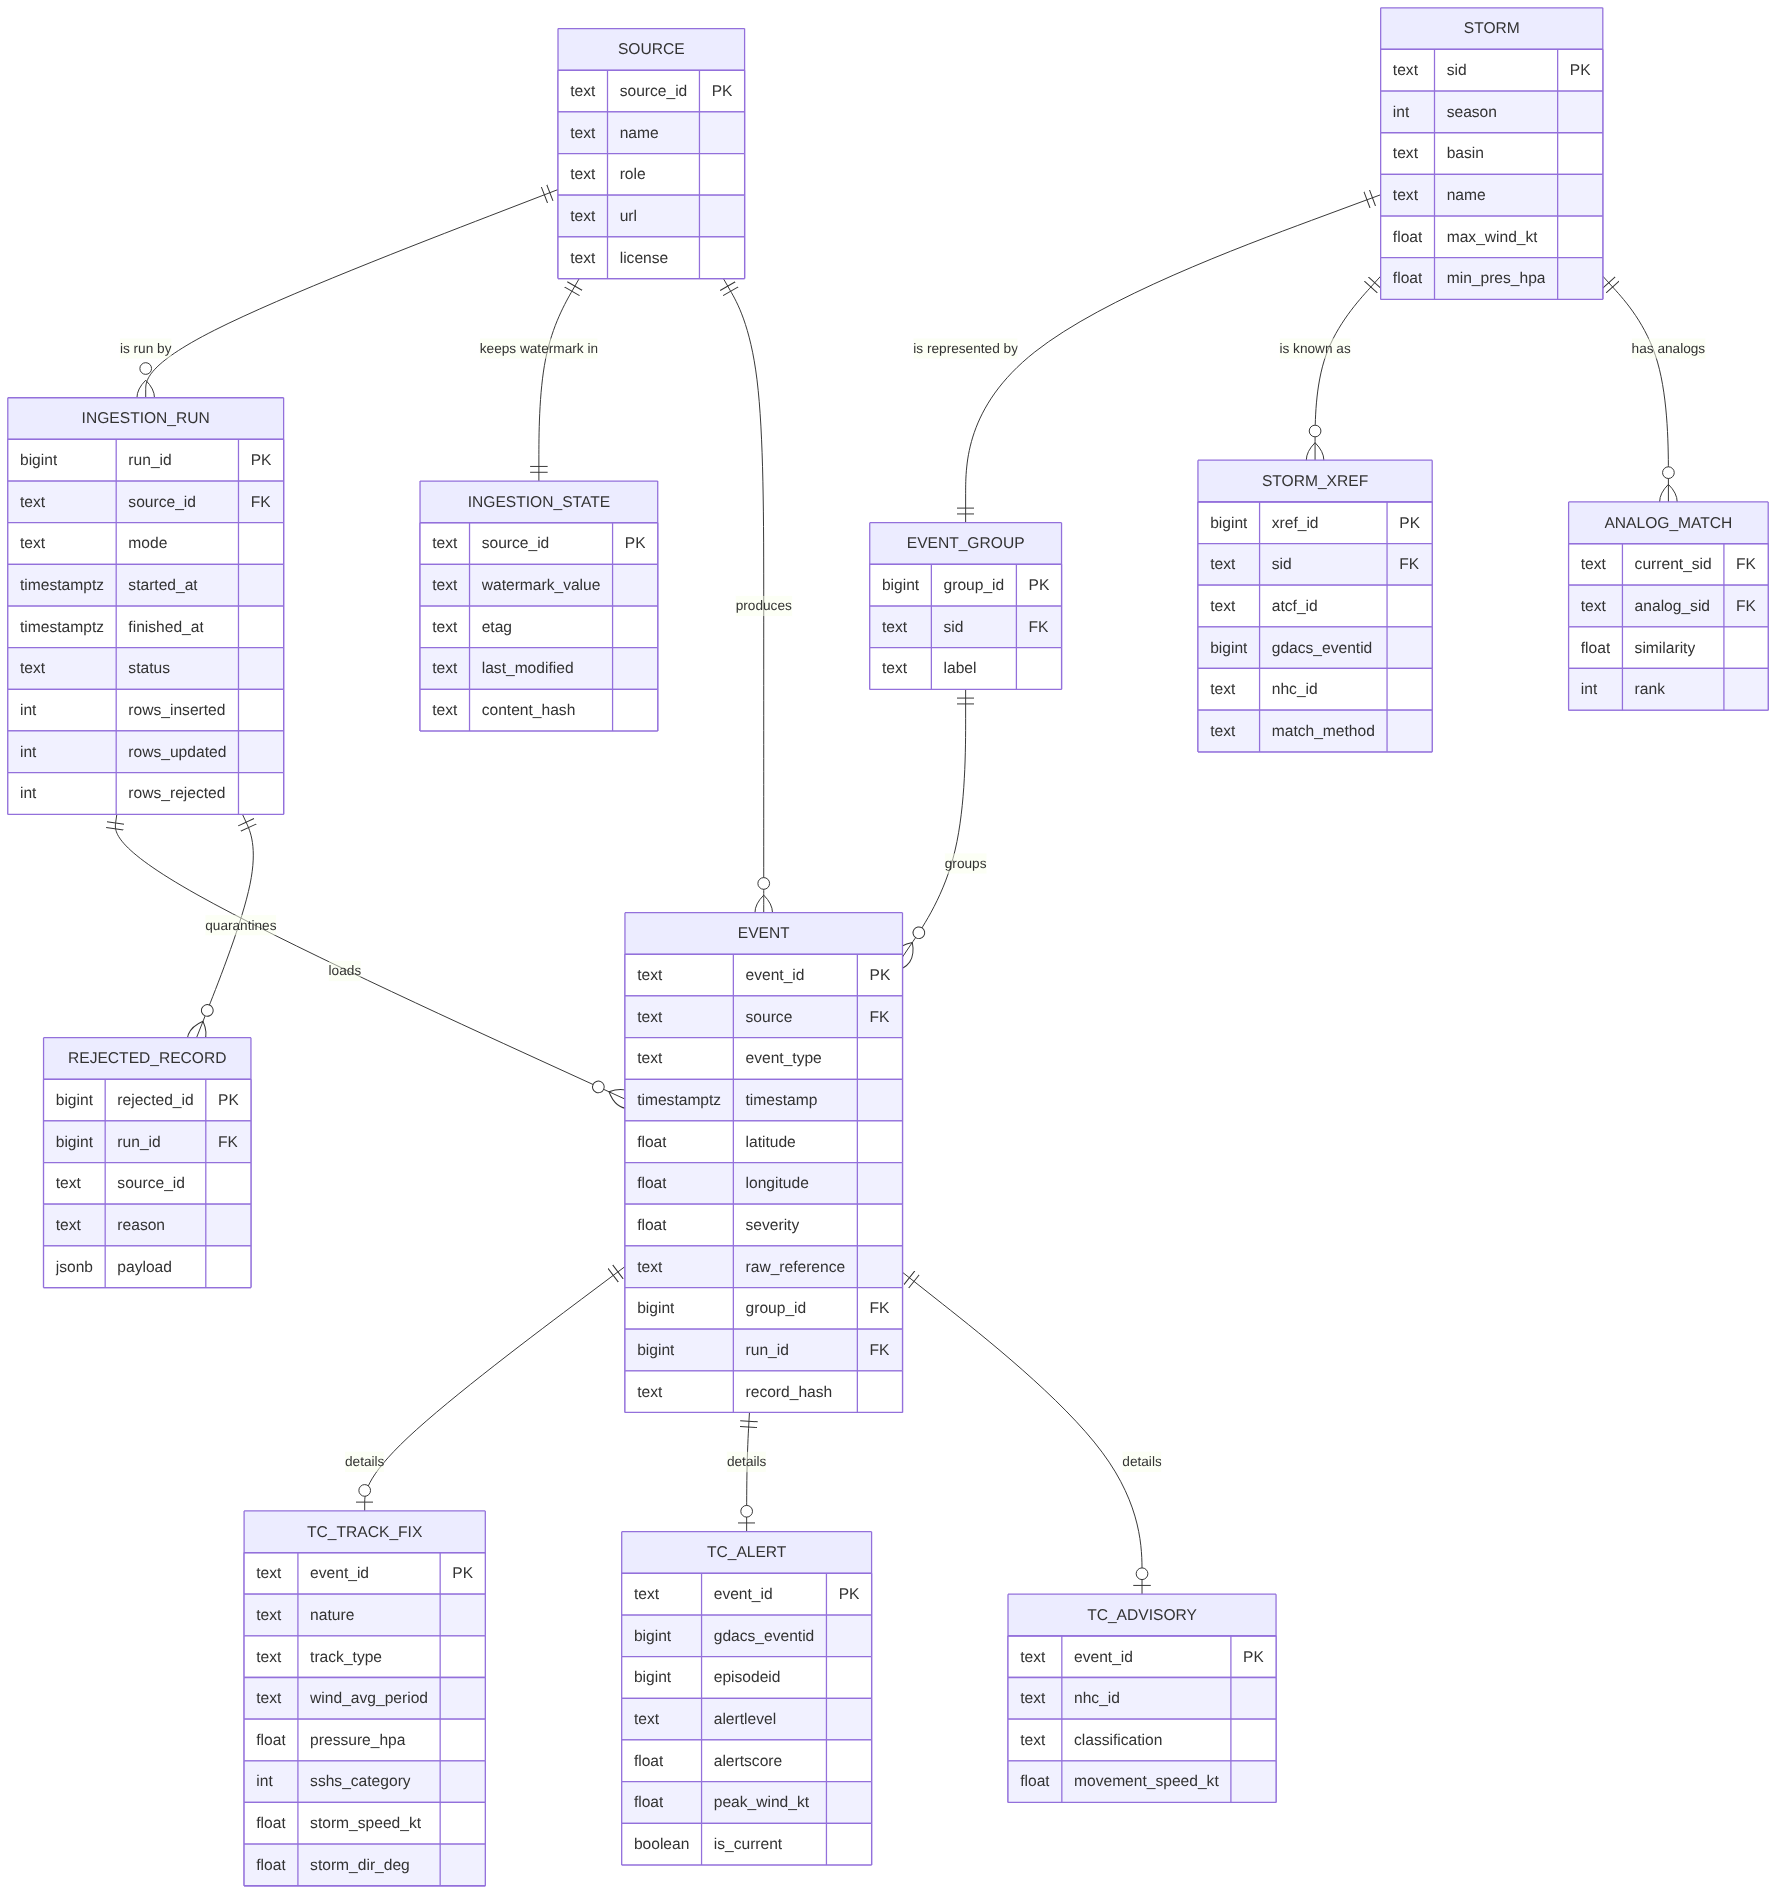
\includegraphics[width=\textwidth,height=0.88\textheight,keepaspectratio]{er_diagram.png}
\caption{First-draft entity--relationship diagram. Common tables follow the course data model; \code{storm}, \code{tc\_track\_fix}, \code{tc\_alert}, \code{tc\_advisory}, \code{storm\_xref} and \code{analog\_match} are the tropical cyclone domain tables.}
\label{fig:er}
\end{figure*}

% ======================= VI. CONTRACT ==============================
\section{Ingestion Contract}\label{sec:contract}

Historical loads are partitioned and idempotent; incremental polls use a watermark and an overlap window, and every write is an upsert on a stable duplicate key, so a repeated run never creates duplicates (Table~\ref{tab:contract}). Both duplicate keys were verified: the IBTrACS key had no duplicates among 312{,}394 fixes, spur tracks included, and the GDACS key exposed the month-boundary repeats described in DQ8.

\begin{table*}[t]
\caption{Ingestion Contract per Source}\label{tab:contract}
\centering\footnotesize
\begin{tabularx}{\textwidth}{@{}L{2.0cm}L{3.7cm}L{3.7cm}L{2.5cm}L{1.6cm}Y@{}}
\toprule
Source & Historical strategy & Incremental strategy & Watermark & Polling / overlap & Duplicate key\\
\midrule
S1 IBTrACS since1980 & One download per release; drop units row; chunked parse; 287 season--basin partitions & Weekly conditional GET; upsert rows whose hash changed & ETag and Last-Modified & Weekly / whole file & (SID, ISO\_TIME)\\
S2 GDACS archive & Monthly windows 2015--present; pages until HTTP 204 & Covered by S4 & Last completed month & One-off & (eventid, episodeid), deduplicated\\
S3 IBTrACS ACTIVE & Not applicable & Conditional GET; upsert all rows on change; storms age out, never deleted & ETag and Last-Modified; SHA-256 fallback & 3 h / 7 days & (SID, ISO\_TIME)\\
S4 GDACS current & Not applicable & Search from watermark minus overlap; changed \code{datemodified} or hash updates the row & Max.\ \code{datemodified} & 1 h / 72 h & (eventid, episodeid)\\
S5 NHC (optional) & Recorded feeds as fixtures & GET with If-None-Match; new \code{lastUpdate} creates a row & ETag, then \code{lastUpdate} & 1 h ($\geq$ 300 s) & (id, lastUpdate)\\
\bottomrule
\end{tabularx}
\end{table*}

Revisions are expected. Provisional IBTrACS fixes are revised in place and replaced on re-analysis, so a SHA-256 hash of each normalized row detects changes for the same key. A fix that disappears from a new release is flagged as withdrawn rather than deleted. GDACS issues a new episode per update and can modify older ones, which is why its watermark is moved back by 72~h before every poll; the observed 37~h delay of CEMPAKA-26 falls inside that window.

The system stays correct if a run fails halfway. Each run opens an \code{ingestion\_run} record and writes the raw response to \code{data/raw} before parsing. Each partition is written in its own transaction, and \code{ingestion\_state} is advanced only in the transaction of the last partition and only if all partitions succeeded. A failed run is marked as such; the next run starts from the unchanged watermark, re-reads the cached file and repeats idempotent upserts. Invalid records are quarantined with their reason and payload without blocking the rest of the partition.

% ======================= VII. PROJECT ==============================
\section{Project Definition}\label{sec:project}

\subsection{Functional User}
The primary user is an emergency-management analyst in a national risk-management office or a humanitarian coordination team. This user reads maps and time series daily, knows the Saffir--Simpson scale and alert levels, is not a programmer, and works under time pressure. The dashboard supports four decisions: whether to escalate the monitoring of a storm, which historical events to use as reference for impacts and response, when to brief decision-makers, and whether the data on screen is fresh enough to act on. Today this requires opening several websites and matching storms by hand.

\subsection{User Stories}
Table~\ref{tab:stories} lists the user stories, prioritized with the MoSCoW method and covering monitoring, analysis and trust.

\begin{table}[t]
\caption{User Stories (MoSCoW)}\label{tab:stories}
\centering\footnotesize
\begin{tabularx}{\columnwidth}{@{}L{0.7cm}L{0.95cm}Y@{}}
\toprule
ID & Priority & As an analyst, I want to \ldots{} so that \ldots\\
\midrule
US-01 & Must & see every active storm on a map with position, intensity and category, so that I know the current situation at a glance\\
US-02 & Must & have storms, fixes and alert changes since my last visit highlighted, so that I notice what is new\\
US-03 & Must & get the five most similar historical storms in the basin with their score, so that I can judge whether the storm is unusual\\
US-04 & Must & see the last successful update and record count per source, so that I know how fresh and complete the data is\\
US-05 & Should & overlay the current track on the analog tracks and intensity curves, so that I can explain the similarity\\
US-06 & Should & see the current motion speed and direction, so that I can describe where the storm is heading\\
US-07 & Should & have provisional and rejected records flagged and counted, so that I know which values may change\\
US-08 & Could & filter the archive by basin, season and peak category, so that I can study the climatology behind an analog\\
US-09 & Could & see the NHC forecast cone for Atlantic and eastern Pacific storms, so that the official outlook sits next to the analogs\\
US-10 & Won't & get projected impacts by country; excluded because impact modelling is out of scope\\
\bottomrule
\end{tabularx}
\end{table}

\subsection{Indicator Proposal: Storm Analog Similarity}
The Storm Analog Similarity (SAS) indicator ranks historical storms by how closely their track and intensity resemble the recent history of the current storm. It describes resemblance and is not a prediction. The inputs are the last 48~h of fixes of the current storm, resampled to 6~h steps, and all storms from 1980 to the previous season in the same basin with \code{TRACK\_TYPE = main} and at least one fix within 300~km of the current position. For each candidate, a 48~h window slides along its track and the window that minimizes
\begin{equation}
D = w_1\frac{\bar{d}_{\mathrm{track}}}{d_0} + w_2\frac{\overline{|\Delta V|}}{V_0} + w_3\frac{\overline{|\Delta\theta|}}{\theta_0} + w_4\frac{|\Delta\mathrm{doy}|}{t_0}
\end{equation}
is kept, and the score is $\mathrm{SAS} = 100\,e^{-D}$. Here $\bar{d}_{\mathrm{track}}$ is the mean great-circle distance between aligned fixes, $\Delta V$ the wind difference, $\Delta\theta$ the heading difference and $\Delta\mathrm{doy}$ the circular day-of-year difference. The starting values are $d_0=250$~km, $V_0=15$~kt, $\theta_0=45^\circ$, $t_0=30$~days and equal weights, all subject to calibration. The dashboard shows the top five analogs with scores between 0 and 100 (provisional bands: 70--100 high, 40--69 moderate, below 40 low) and the percentile of the current intensity among them.

The indicator will be validated against historical events in four ways: a hindcast in which storms of a held-out season are truncated after 48~h and their analogs are compared with random storms of the same basin; a review of well-documented storms to check that analogs share basin, latitude band and motion regime; a sensitivity analysis that varies each weight by $\pm50\,\%$ and measures the overlap of the top-five lists; and a stability check across successive provisional updates of active storms.

% ======================= VIII. RISKS ===============================
\section{Risks and Mitigation}\label{sec:risks}

Table~\ref{tab:risks} lists the risks identified during source validation. The most likely are empty incremental feeds off-season, ambiguous identifiers and provisional revisions; the most damaging would be a schema change or a misreading of the GDACS severity.

\begin{table}[t]
\caption{Risks and Mitigation}\label{tab:risks}
\centering\footnotesize
\begin{tabularx}{\columnwidth}{@{}L{0.55cm}L{2.45cm}c Y@{}}
\toprule
ID & Risk & L / I & Mitigation\\
\midrule
R1 & Source outage & M / H & Retries with back-off; cached raw files; staleness banner\\
R2 & Rate limiting (none published) & L / M & 1 req/s, descriptive User-Agent, cached pages\\
R3 & Schema change or column reordering & M / H & Columns read by name; schema check; quarantine; fixtures\\
R4 & License or attribution breach & L / H & Attribution per source in configuration, dashboard and report\\
R5 & Data volume (145~MB, 288 requests) & M / M & since1980 subset; chunked load; 287 partitions\\
R6 & Ambiguous identifiers across sources & H / H & \code{storm\_xref}; spatio-temporal matching (83\,\% in 2024)\\
R7 & Empty feeds off-season & H / M & Global scope; empty response is success; replay fixtures\\
R8 & Provisional data revised & H / M & Row hash, overlap windows, provisional flag\\
R9 & Mixed averaging periods & H / M & Store period; prefer 1-min wind; same-basin analogs\\
R10 & GDACS severity read as current & M / H & Stored as peak wind; intensity from IBTrACS only\\
\bottomrule
\multicolumn{4}{@{}l}{\scriptsize L / I: likelihood / impact (L low, M medium, H high).}
\end{tabularx}
\end{table}

% ======================= IX. ARCHITECTURE ==========================
\section{System Architecture and Repository}\label{sec:arch}

Fig.~\ref{fig:arch} shows the target architecture, which follows the common technical contract of the course: a Docker Compose stack with the database, the ingestion application, an orchestrator and the Plotly Dash dashboard, configured through environment variables and a source registry file. Raw responses land first, are normalized and validated, and only then reach the database; invalid records are quarantined.

\begin{figure*}[tp]
\centering
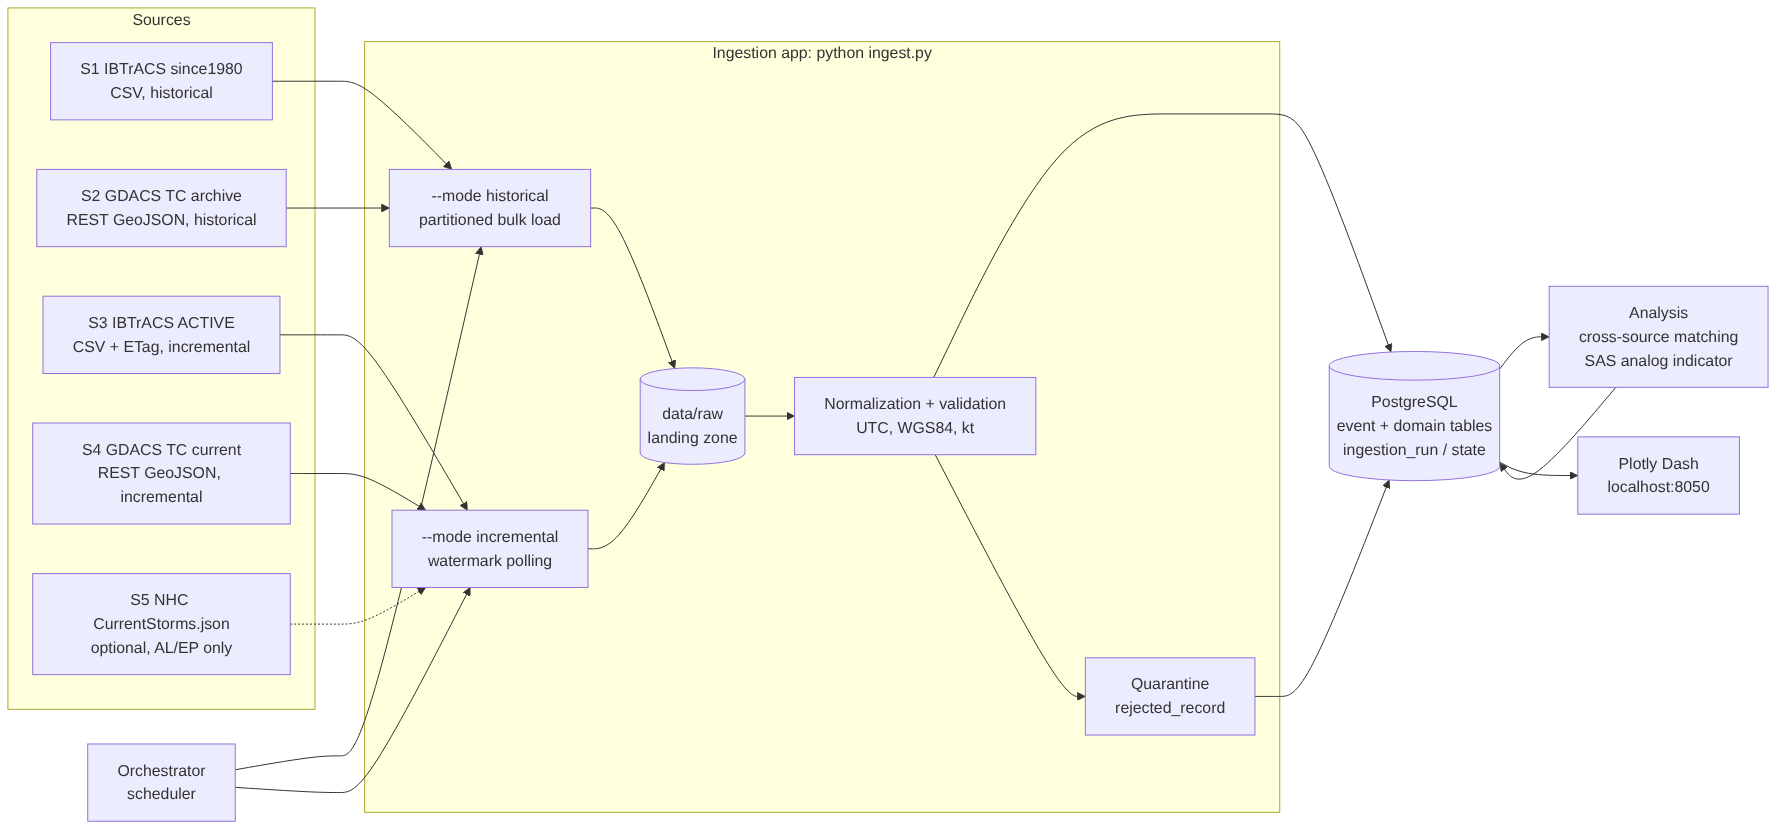
\includegraphics[width=0.92\textwidth]{architecture.png}
\caption{Target architecture. Historical and incremental sources feed the two modes of \code{ingest.py}; raw responses land in \code{data/raw}, are normalized and validated, and reach PostgreSQL or the quarantine table; the analysis layer and the dashboard read from the database. The dotted line marks the optional NHC source.}
\label{fig:arch}
\end{figure*}

The repository (\repourl) follows the required structure: an ingestion package under \code{src/} with source adapters, normalization and storage modules; the command-line stub \code{ingest.py} with historical and incremental modes; \code{config/sources.yaml} with one entry per source; the git-ignored landing zone \code{data/raw/}; the draft schema in \code{sql/}; the dashboard stub in \code{dashboard/}; tests with recorded responses in \code{tests/fixtures/}; and the folders \code{notebooks/}, \code{docs/} and \code{workshop\_1/}, which hold the executed profiling notebook, the raw samples, the evidence files, the mapping table and the source-status log. Twenty-eight automated tests pass, four of them on the responses recorded for this report.

% ======================= X. OPEN ISSUES ============================
\section{Open Issues and Conclusion}\label{sec:open}

Four points will be confirmed with the instructor: whether IBTrACS and GDACS, each used as one historical and one incremental source as in the team assignment, count as four sources; whether GDACS is accepted as the second historical source given that its archive is usable only from about 2015; whether the global scope with same-basin analogs and the 1980 baseline are accepted; and whether a two-poll comparison without changes is sufficient or a third poll after the next IBTrACS release should be included.

All four sources are accessible, documented and profiled with real responses. The validation changed three design decisions: GDACS severity is stored as peak wind rather than current intensity, the GDACS archive is used from 2015, and the GDACS watermark relies on \code{datemodified} with a 72~h overlap because the API sends no HTTP validators. These decisions, the canonical model and the ingestion contract are the basis for the historical ingestion of Workshop~2.

% ======================= REFERENCES ================================
\balance
\begin{thebibliography}{10}
\footnotesize
\setlength{\itemsep}{1pt}

\bibitem{ws1}
C.~A. Sierra, ``Workshop No.~1: Hazard definition, source validation, and data contract,'' Data Analysis Programming, Universidad Distrital Francisco José de Caldas, Bogotá, Colombia, 2026.

\bibitem{teams}
C.~A. Sierra, ``Team project assignment: Natural hazard monitoring systems,'' Data Analysis Programming, Universidad Distrital Francisco José de Caldas, Bogotá, Colombia, 2026.

\bibitem{ibtracs-paper}
K.~R. Knapp, M.~C. Kruk, D.~H. Levinson, H.~J. Diamond, and C.~J. Neumann, ``The International Best Track Archive for Climate Stewardship (IBTrACS): Unifying tropical cyclone best track data,'' \emph{Bull. Amer. Meteor. Soc.}, vol.~91, pp.~363--376, 2010, doi: 10.1175/2009BAMS2755.1.

\bibitem{ibtracs-data}
J.~Gahtan, K.~R. Knapp, C.~J. Schreck~III, H.~J. Diamond, J.~P. Kossin, and M.~C. Kruk, ``International Best Track Archive for Climate Stewardship (IBTrACS) Project, Version 4.01,'' NOAA National Centers for Environmental Information, 2024, doi: 10.25921/82ty-9e16. Accessed: Nov.~14, 2026.

\bibitem{ibtracs-cols}
NOAA National Centers for Environmental Information, ``IBTrACS v04r01 column documentation,'' 2025. [Online]. Available: \url{https://www.ncei.noaa.gov/sites/default/files/2025-09/IBTrACS_v04r01_column_documentation.pdf}

\bibitem{ibtracs-tech}
NOAA National Centers for Environmental Information, ``International Best Track Archive for Climate Stewardship (IBTrACS): Technical documentation, version 4r01,'' Apr. 2025. [Online]. Available: \url{https://www.ncei.noaa.gov/sites/default/files/2025-04/IBTrACS_version4r01_Technical_Details.pdf}

\bibitem{gdacs-api}
Global Disaster Alert and Coordination System, ``GDACS API quick start,'' European Commission Joint Research Centre and UN OCHA, 2025. [Online]. Available: \url{https://www.gdacs.org/gdacsapi/}

\bibitem{nhc-json}
NOAA National Hurricane Center, ``Tropical cyclone status JSON file reference.'' [Online]. Available: \url{https://www.nhc.noaa.gov/productexamples/NHC_Tropical_Cyclone_Status_JSON_File_Reference.pdf}

\bibitem{sshws}
NOAA National Hurricane Center, ``Saffir--Simpson hurricane wind scale.'' [Online]. Available: \url{https://www.nhc.noaa.gov/aboutsshws.php}

\end{thebibliography}

\end{document}
